\chapter{Modelagem das Funções do Receptor}
A caracterização do arcabouço estrutural utilizando métodos sismológicos possui problemas de unicidade de solução, como outros métodos geofísicos.  Essa falta de informação direta do objeto em estudo proporciona uma gama de soluções, entretante há inúmeros meios de se contornar essa situação. A modelagem mostra-se uma boa opção, pois consegue comprovar se a técnica utilizada tem resolução para seu objetivo.

\begin{figure}[!ht]
\centering
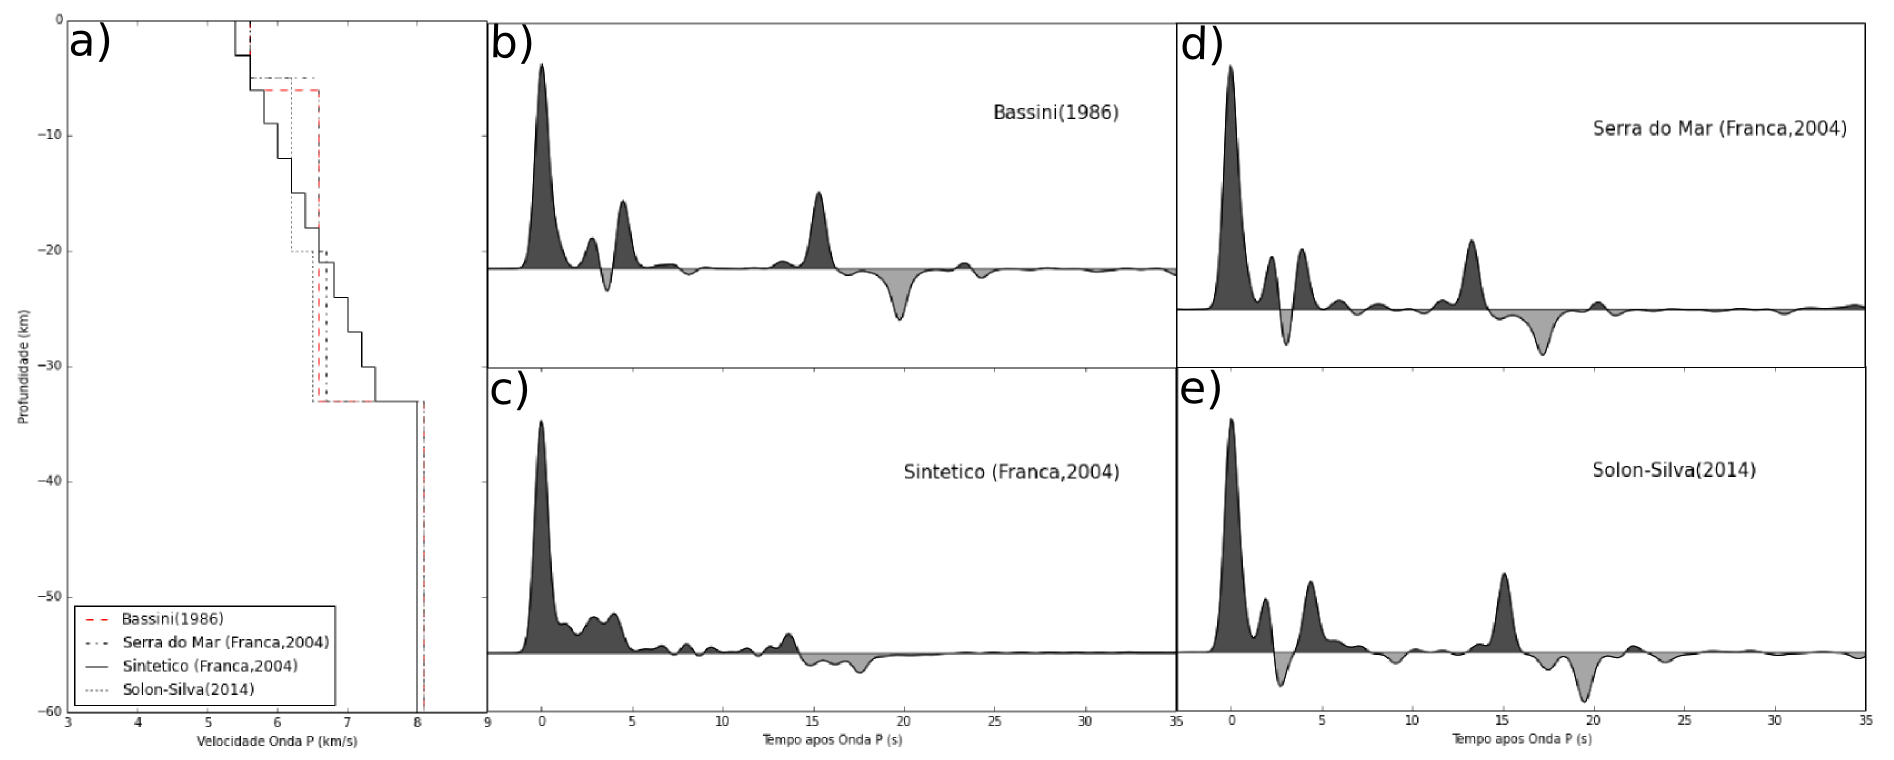
\includegraphics[scale=0.25]{modelagem_RF.png}
\caption{Funções do Receptor Sintéticas para área abrangida pelo projeto do SUBSAL segundo vários tipos de modelos de velocidade da onda P.}
\label{modelagem}
\end{figure}

Para delimitar as principais feições estruturais da área em estudo fez o uso de modelos simples, como visto na Figura \ref{modelagem}-a, apenas com camadas planas, porém tais modelos são condizentes com o contexto geológico local. Com esses modelos pretende-se mostrar que as estimativas da espessura crustal e razão $V_{p}/V_{s}$ são consistentes com os dados observados. Para a confecção e cálculo das Funções do Receptor Sintéticas aplicou-se a metodologia proposta por \cite{Ammon_waterlevel_1997}. 

Os programas utilizados para criar os modelos de velocidade da onda $P$ foram "\textit{icmod}" e "\textit{vplot[s]}". A preparação dos dados sintéticos foi feita pelo programa "\textit{respknt}". O programa "\textit{pwaveqn}" calculou as Funções do Receptor no domínio da frequência para os modelos pré-estabelecidos. Os parâmetros utilizados para o cálculo das Funções do Receptor estão na Figura \ref{modelagem}. Toda a demonstração da modelagem e cálculo das Funções do Receptor sintéticas está disponibilizada por \cite{Ammon_waterlevel_1997} em \url{http://eqseis.geosc.psu.edu/~cammon/HTML/RftnDocs/rftn01.html}.

Os modelos de velocidade da onda P ($V_{p}$) são exemplos retirados da literatura sobre a região em estudo, \ref{modelagem}-a. \cite{Bassini_1986} foi o primeiro a estimar a estrutura crustual para a região da Faixa Riberia, então neste trabalho utilizou-se o modelo de velocidade sísmica para a região da Serra do Mar, como observado na Figura \ref{modelagem}-b. Mais tarde, \cite{sand_franca_crustal_2004} re-compilou os dados de \cite{Bassini_1986} e propôs um novo modelo de velocidade sísmica da região da Serra do Mar, como visto na Figura \ref{modelagem}-d. Recentemente \cite{flora_solon_ancient_2013} e \cite{Silva_2014} geraram resultados da estrutura crustal reginal através dos métodos magnetométrico e gravimétrico, respectivamente. Baseando-se nesses resultados, organizou-se um modelo de velocidade sísmica para a região em estudo, como visto na Figura \ref{modelagem}-e. Uma outra opção de modelo sísmico levantada por \cite{sand_franca_crustal_2004} é o modelo Sintético, mostrado na Figura \ref{modelagem}-c. Neste modelo o autor considera que a variação das propriedades físicas da região aumenta progressivamente com a profundidade.

\begin{figure}[!ht]
\centering
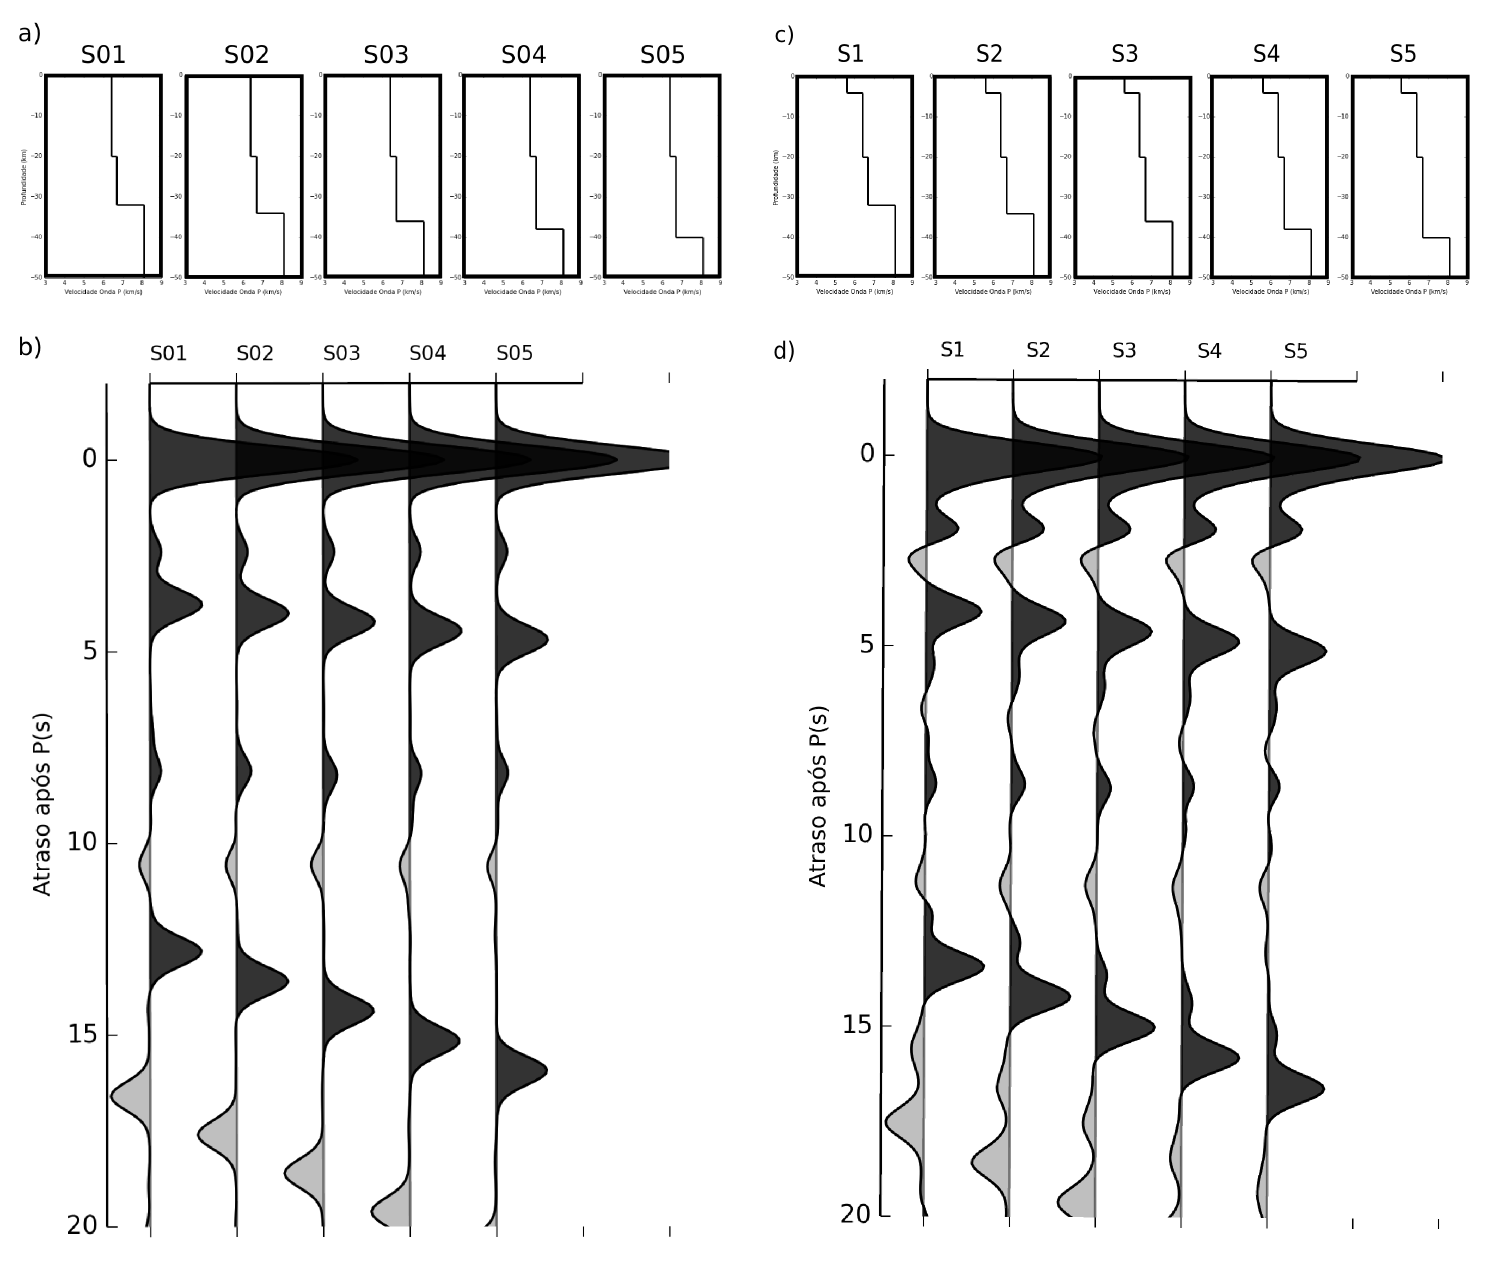
\includegraphics[scale=0.25]{perfil_RF_sintetico.png}
\caption{Perfil com Funções do Receptor Sintéticas para área abrangida pelo projeto do SUBSAL segundo modelos de velocidade Solon-Silva(2014).}
\label{modelagem}
\end{figure}

As Funções do Receptor sintéticas apresentadas na Figura \ref{modelagem} mostram uma reflexão característica por volta de 5 segundos, está é a primeira reflexão de Moho, onde a onda P se converte em S. Antes dessa reflexão é notável um pulso senoidal em torno de 2.5 segundos nas Figuras \ref{modelagem}-b, \ref{modelagem}-d e \ref{modelagem}-e. Este pulso está relacionado com a camada superficial de baixa velocidade. Tal camada possui espessura aproximada de 5 quilômetros, esta representa a Bacia de Taubaté na região da Faixa Ribeira. As outras reverberações são bem características, As multiplas $PpPs$ e $PpSs+PsPs$ são bem demarcadas em $\sim 13$ e $\sim 19$ segundos, respectivamente.